
\section{\label{sec:moreConvergenceDiagrams}Diagram Kekonvergenan Lainnya}

Fungsi kubik $g(x)=1-x^{3}$ memiliki satu akar riil, $1$. Namun,
fungsi tersebut juga memiliki dua akar kompleks. Jika Anda telah mempelajari
analisis kompleks, Anda mungkin sudah mengetahui kedua akar lainnya.
Bahkan jika belum, Anda dapat menentukannya dengan teknik dasar prakalkulus.
Karena $1$ merupakan akar, Anda dapat menggunakan pembagian sintetis
untuk melakukan deflasi pada polinom:

\begin{center}
\begin{tabular}{ccccc}
\multicolumn{1}{c|}{$1$} & $-1$ & $0$ & $0$ & $1$\tabularnewline
\cline{1-1}
 &  & $-1$ & $-1$ & $-1$\tabularnewline
\hline 
 & $-1$ & $-1$ & \multicolumn{1}{c|}{$-1$} & \multicolumn{1}{c|}{$0$}\tabularnewline
\cline{5-5}
\end{tabular}
\par\end{center}

\noindent Pembagian ini menunjukkan bahwa $g(x)=(x-1)(-x^{2}-x-1)$,
sehingga kedua akar lainnya merupakan solusi persamaan $-x^{2}-x-1=0$;
dengan demikian, persoalannya tereduksi menjadi persamaan kuadrat.
Solusinya adalah $\frac{1\pm\sqrt{1-4}}{-2}=-\frac{1}{2}\pm i\frac{\sqrt{3}}{2}$.
Selain itu, Anda mungkin mengenali $1-x^{3}$ sebagai salah satu bentuk
khusus polinom, yakni selisih dua kubus. 

Tentu saja semua ini menarik, tetapi apa hubungannya dengan analisis
numerik? Mungkin mengejutkan bahwa iterasi titik tetap (dan karena
itu metode Newton), metode sekan, serta metode Steffensen dapat digunakan
untuk menemukan akar kompleks sama baiknya dengan akar riil! Bahkan
algoritmenya tidak perlu dimodifikasi! Namun, bahasa pemrograman yang
digunakan untuk menerapkan metode-metode tersebut harus mampu menangani
aritmetika bilangan kompleks. Octave mendukungnya secara langsung.

Pertama, mencari akar $g(x)=1-x^{3}$ setara dengan mencari titik
tetap $f(x)=1/x^{2}$. Mengapa? Lihat jawabannya \vpageref{que:whyEquivalent}.
Dengan menetapkan $x_{0}=-1+i$ lalu menerapkan metode Newton dan
metode sekan pada $g(x)=1-x^{3}$, serta metode Steffensen pada $f(x)=1/x^{2}$
kita memperoleh hasil berikut:

\begin{center}
\begin{tabular}{c|ccc}
 & \multicolumn{3}{c}{$x_{i}$}\tabularnewline
\cline{2-4}
$i$ & Steffensen & Sekan & Newton\tabularnewline
\hline 
$0$ & $-1+i$ & $-1+i$ & $-1+i$\tabularnewline
$1$ & $-0.85+0.8i$ & $-0.66666666+0.83333333i$ & $-0.66666666+0.83333333i$\tabularnewline
$2$ & $-0.60313824+0.67770639i$ & $-0.55034016+0.82376444i$ & $-0.50869191+0.84109987i$\tabularnewline
$3$ & $-0.39846066+0.84671567i$ & $-0.49763752+0.85554014i$ & $-0.49932999+0.86626917i$\tabularnewline
$4$ & $-0.51660491+0.84998590i$ & $-0.49932718+0.86627140i$ & $-0.49999991+0.86602490i$\tabularnewline
$5$ & $-0.49910537+0.86543351i$ & $-0.50000774+0.86602504i$ & $-0.50000000+0.86602540i$\tabularnewline
$6$ & $-0.50000228+0.86602568i$ & $-0.49999999+0.86602540i$ & \tabularnewline
$7$ & $-0.50000000+0.86602540i$ & $-0.50000000+0.86602540i$ & \tabularnewline
$8$ & $\vdots$ & $\vdots$ & $\vdots$\tabularnewline
\end{tabular}
\par\end{center}

\noindent Setiap barisan dengan cepat konvergen ke akar kompleks $-\frac{1}{2}+\frac{\sqrt{3}}{2}i$.
Ini bukan kebetulan ataupun contoh yang dibuat-buat. Secara umum,
metode-metode ini bekerja sama baiknya di bidang kompleks maupun pada
garis riil. Kita pun dapat menemukan akar riil dengan memulai dari
bilangan kompleks. Sebagai contoh, jika nilai awal $x_{0}$ diubah
menjadi $1+i$, metode Newton konvergen ke $1$.

Setelah memperluas cakupan metode-metode ini ke bilangan kompleks,
kini ada jenis diagram kekonvergenan baru yang perlu dipertimbangkan.
Kita dapat mengamati pola kekonvergenan ketiga metode untuk banyak
nilai awal di bidang kompleks, bukan hanya pada garis riil. Gambar
\ref{fig:complexConvergenceDiagram1} menampilkan diagram kekonvergenan
metode Newton dengan $g(x)=1-x^{3}$, metode sekan dengan satu nilai
awal untuk $g(x)=1-x^{3}$, dan metode Steffensen dengan $f(x)=1/x^{2}$.
\begin{figure}
\caption{\label{fig:complexConvergenceDiagram1}Diagram kekonvergenan pada
bidang kompleks.}

\begin{centering}
\begin{tabular}{cc}
\multirow{3}{5cm}{\textbf{Urutan dari atas ke bawah:}\\
metode Newton dengan
\[
g(x)=1-x^{3}
\]
dan dwell 20;\\
metode sekan dengan satu nilai awal untuk
\[
g(x)=1-x^{3}
\]
dan dwell 40;\\
metode Steffensen dengan
\[
f(x)=\frac{1}{x^{2}}
\]
dan dwell 40.\\
Setiap diagram mencakup bagian bidang kompleks dengan bagian riil
dalam $[-5,5]$ dan bagian imajiner dalam $[-3.75,3.75]$.} & \includegraphics[scale=0.4]{figures/convergenceDiagram1\lyxdot 1}\tabularnewline
 & \includegraphics[scale=0.4]{figures/convergenceDiagram1\lyxdot 2a}\tabularnewline
 & \includegraphics[scale=0.4]{figures/convergenceDiagram1\lyxdot 3}\tabularnewline
\end{tabular}
\par\end{centering}
\end{figure}
Setiap diagram mencakup bagian bidang kompleks dengan bagian riil
dalam $[-5,5]$ dan bagian imajiner dalam $[-3.75,3.75]$. Sudut kiri
atas setiap diagram mewakili nilai awal $-5+3.75i$ sedangkan sudut
kanan bawah mewakili nilai awal $5-3.75i$. Pusat setiap diagram mewakili
nilai awal $0$. Warna-warna tersebut bersesuaian dengan ketiga akar:
merah dengan $1$, hijau dengan $-\frac{1}{2}+\frac{\sqrt{3}}{2}i$,
dan biru dengan $-\frac{1}{2}-\frac{\sqrt{3}}{2}i$. Hitam menandakan
kegagalan mencapai kekonvergenan. Perbedaan intensitas warna merah,
hijau, dan biru menunjukkan jumlah iterasi yang diperlukan metode
untuk konvergen. Semakin tinggi intensitas, semakin sedikit iterasinya.
Untuk $x_{0}=5-3.75i$, terlihat bahwa metode Newton dan metode sekan
dengan satu nilai awal sama-sama konvergen ke $-\frac{1}{2}+\frac{\sqrt{3}}{2}i$,
karena sudut kanan atas setiap diagram berwarna hijau. Sebaliknya,
metode Steffensen gagal konvergen ke akar mana pun jika dimulai dari
$x_{0}=5-3.75i$, sebagaimana ditunjukkan oleh warna hitam di sudut
kanan atas diagram kekonvergenan.

Dwell menyatakan jumlah maksimum iterasi yang diperbolehkan. Jadi,
titik-titik hitam sebenarnya mewakili nilai awal yang belum mencapai
kekonvergenan dalam jumlah iterasi yang tidak melebihi dwell. Ini
berbeda dengan menyatakan bahwa metode tersebut sama sekali tidak
konvergen untuk nilai-nilai awal itu. Sebagian nilai awal yang ditampilkan
hitam mungkin tetap menghasilkan kekonvergenan jika diberi lebih banyak
iterasi.

Ada dua hal yang sangat mencolok pada diagram kekonvergenan ini. Pertama,
metode sekan dengan satu nilai awal dan metode Newton konvergen untuk
himpunan nilai awal yang jauh lebih besar daripada metode Steffensen.
Hal ini, setidaknya sebagian, disebabkan oleh fungsi yang dipilih.
Untuk fungsi lain, mungkin ada skema titik tetap yang membuat metode
Steffensen konvergen pada himpunan nilai awal yang besar pula. Kedua,
pola warnanya sangat rumit, bahkan bersifat fraktal. Memprediksi akar
mana yang akan dicapai suatu metode untuk nilai awal tertentu---dan
bahkan apakah metode itu akan konvergen sama sekali---merupakan persoalan
yang sangat sulit! Padahal analisis ini dilakukan pada fungsi yang
cukup sederhana.

Sekarang pertimbangkan persoalan yang jauh lebih rumit---mencari
akar $g(z)=e^{z}-z$ atau, secara ekuivalen, mencari titik tetap $f(z)=e^{z}$.
Grafik $f(z)$ pada bilangan riil akan segera meyakinkan Anda bahwa
tidak ada solusi riil. Diperlukan pemikiran lebih lanjut untuk menentukan
sifat solusi kompleksnya.

Untuk itu, tetapkan bilangan riil $a_{0}$ dan tinjau garis vertikal
di bidang kompleks, $L_{a_{0}}=\{a_{0}+ib:b\in\mathbb{R}\}$. Citra
$L_{a_{0}}$ oleh fungsi eksponensial adalah sebuah lingkaran berjari-jari
$e^{a_{0}}$ yang berpusat di titik asal. Memang, $e^{a_{0}+ib}=e^{a_{0}}e^{ib}=e^{a_{0}}(\cos b+i\sin b)$.
Jadi, $b$ memparameterkan lingkaran yang berpusat di titik asal dengan
jari-jari $e^{a_{0}}$. Sekarang, misalkan $L_{a_{0}}$ memuat sebuah
titik tetap, $\hat{z}=a_{0}+i\hat{b}$, dari fungsi eksponensial,
$f(z)=e^{z}$. Maka $\hat{z}=f(\hat{z})$, atau $a_{0}+i\hat{b}=e^{a_{0}}(\cos\hat{b}+i\sin\hat{b})$.
Kita menyimpulkan bahwa garis dan lingkaran tersebut berpotongan di
titik tetap itu. Setiap titik tetap $f$ niscaya merupakan titik potong
antara garis $L_{a_{0}}$ dan lingkaran $C_{a_{0}}$ untuk suatu $a_{0}$.
Gambar 
\begin{figure}
\caption{\label{fig:verticalLineAndCircle}Sebuah garis vertikal dan citranya
oleh fungsi eksponensial.}

\centering{}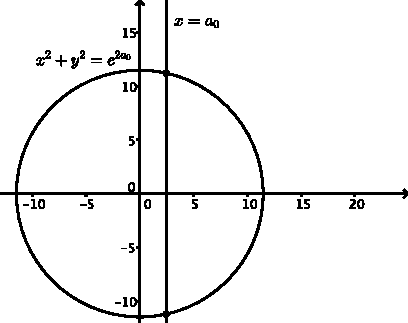
\includegraphics{figures/roots-more2}
\end{figure}
\ref{fig:verticalLineAndCircle} memperlihatkan contoh yang mewakili.
Faktanya, diagram tersebut memperlihatkan kasus yang menarik: $x=a_{0}\approx2.439940377216816$.
Koordinat kedua titik potong adalah 
\[
(2.439940377216816,\pm11.2098911414971).
\]
Hal menariknya ialah 
\[
e^{2.439940377216816+11.2098911414971i}\approx2.439940377216816-11.2098911414971i
\]
dan 
\[
e^{2.439940377216816-11.2098911414971i}\approx2.439940377216816+11.2098911414971i.
\]
Kedua titik tersebut saling menjadi citra satu sama lain oleh fungsi
eksponensial! Titik-titik yang kita temukan di sini disebut titik
periodik. Jika kita tetapkan $z_{1}=2.439940377216816-11.2098911414971i$
dan $z_{2}=2.439940377216816+11.2098911414971i$, maka $e^{z_{1}}=z_{2}$
dan $e^{z_{2}}=z1$. Oleh karena itu, jika kita melakukan iterasi
$z_{2}=f(z_{1})$, $z_{3}=f(z_{2})$, $z_{4}=f(z_{3})$, $z_{5}=f(z_{4})$,
dan seterusnya, barisan $z_{1},z_{2},z_{3},z_{4},\ldots$ sebenarnya
berbentuk
\[
z_{1},z_{2},z_{1},z_{2},z_{1},z_{2},\ldots.
\]
Barisan itu hanya bolak-balik antara $z_{1}$ dan $z_{2}$ secara
periodik. Nilai-nilai seperti ini kita sebut titik berperiode 2. Nilai-nilai
tersebut bukan titik tetap $f(z)$ tetapi merupakan titik tetap $f(f(z))$! 

\begin{digression}{Titik periodik.}

\noindent Jika suatu barisan $\langle p_{n}\rangle$ berbentuk
\[
p_{1},p_{2},\ldots,p_{k},p_{1},p_{2},\ldots,p_{k},p_{1},\ldots,\qquad k>1
\]
maka $p_{1}$ disebut titik berperiode $k$ (demikian pula $p_{2},p_{3},\ldots,p_{k}$!). 

\end{digression}

Sebaliknya, $\hat{z}=2.062277729598284+7.588631178472513i$ merupakan
titik tetap (secara hampiran) dari $f(z)$ karena
\[
e^{2.062277729598284+7.588631178472513i}=2.062277729598284+7.588631178472513i.
\]
Selain itu, konjugat $\hat{z}$, yaitu $\overline{\hat{z}}=2.0622377729598284-7.588631178472513i$
juga merupakan titik tetap. Periksalah dengan kalkulator atau Octave!

Secara umum, jika $\hat{z}$ merupakan titik tetap dari $e^{z}$ maka
$\overline{\hat{z}}$ juga merupakan titik tetap:
\[
\hat{z}=e^{\hat{z}}\implies\overline{\hat{z}}=\overline{e^{\hat{z}}}=e^{\overline{\hat{z}}}.
\]
Jadi, ketika kita menemukan satu titik tetap, sebenarnya kita menemukan
dua: titik tetap tersebut dan konjugatnya. 

Kita kini siap kembali meninjau titik-titik potong $L_{a_{0}}$ dan
$C_{a_{0}}$. Anggap $a_{0}+ib$ merupakan titik tetap dari $e^{z}$.
Maka $a_{0}+ib=e^{a_{0}+ib}=e^{a_{0}}(\cos b+i\sin b$), sehingga
\begin{eqnarray}
a_{0} & = & e^{a_{0}}\cos b\nonumber \\
b & = & e^{a_{0}}\sin b\label{eq:expFixedPoint}
\end{eqnarray}
\begin{figure}
\caption{\label{fig:complexConvergenceDiagram2}Diagram kekonvergenan lainnya
pada bidang kompleks.}

\begin{centering}
\includegraphics[scale=0.4]{figures/convergenceDiagram2\lyxdot 1}
\includegraphics[scale=0.4]{figures/convergenceDiagram2\lyxdot 2}
\includegraphics[scale=0.4]{figures/convergenceDiagram2\lyxdot 3} 
\par\end{centering}
\textbf{Urutan dari kiri ke kanan:} metode Newton dengan $g(z)=z-e^{z}$
dan dwell 20; metode sekan dengan $g(z)=z-e^{z}$ dan dwell 40; metode
Steffensen dengan $f(z)=e^{z}$ dan dwell 40. Setiap diagram mencakup
bagian bidang kompleks dengan bagian riil dalam $[-10,30]$ dan bagian
imajiner dalam $[0,73]$.
\end{figure}
Sekarang, karena $a_{0}+ib$ merupakan titik potong, titik itu terletak
pada $C_{a_{0}}$, sehingga $a_{0}^{2}+b^{2}=e^{2a_{0}}\Rightarrow b=\pm\sqrt{e^{2a_{0}}-a_{0}^{2}}$.
Terakhir, dengan menyubstitusikan $b=\sqrt{e^{2a_{0}}-a_{0}^{2}}$
ke \ref{eq:expFixedPoint}, kita memperoleh bahwa suatu titik potong
merupakan titik tetap jika dan hanya jika
\begin{eqnarray}
a_{0} & = & e^{a_{0}}\cos\sqrt{e^{2a_{0}}-a_{0}^{2}}\nonumber \\
 &  & \mbox{dan}\nonumber \\
\sqrt{e^{2a_{0}}-a_{0}^{2}} & = & e^{a_{0}}\sin\sqrt{e^{2a_{0}}-a_{0}^{2}}.\label{eq:realPartRequirement}
\end{eqnarray}
Luangkan waktu untuk memikirkan mengapa  $b=-\sqrt{e^{2a_{0}}-a_{0}^{2}}$
tidak perlu disubstitusikan ke \ref{eq:expFixedPoint}. Petunjuk:
lakukan substitusi dan sederhanakan. Anda akan mendapati bahwa kedua
persamaan yang diperoleh ekuivalen dengan persamaan-persamaan dalam
\ref{eq:expFixedPoint}.

Sebagai contoh, $2.439940377216816-11.2098911414971i$ dan $2.062277729598284+7.588631178472513i$
sama-sama memenuhi persamaan pertama dalam \ref{eq:realPartRequirement},
tetapi $2.439940377216816-11.2098911414971i$ tidak memenuhi persamaan
kedua, sedangkan $2.062277729598284+7.588631178472513i$ memenuhinya.
Jadi, seperti diamati sebelumnya, $2.439940377216816-11.2098911414971i$
bukan titik tetap, tetapi $2.062277729598284+7.588631178472513i$
adalah titik tetap. 

Apakah Anda mengenali persamaan pertama dalam \ref{eq:realPartRequirement}?
Kita pertama kali melihatnya \vpageref{interestingNewton} pada Bagian
\ref{sec:newtonsMethod}. Seperti dicatat di sana, lima solusi terkecil
adalah
\[
\begin{gathered}.3181315052047641,\ 1.668024051576096,\ 2.062277729598284,\\
2.439940377216816,\ 2.653191974038697,\ldots
\end{gathered}
\]
Nilai $2.062277729598284$ dan $2.439940377216816$ menjadi contoh
dalam pembahasan ini. Bagaimana dengan tiga nilai lainnya dalam daftar
tersebut? Apakah nilai-nilai itu menghasilkan titik tetap fungsi eksponensial?
Titik berperiode dua? Atau sesuatu yang lain? Luangkan waktu untuk
menyelidikinya. Jawabannya \vpageref{que:natureOfRoots}. Penyelidikan
dengan Octave terhadap $2.062277729598284$, yang kita ketahui merupakan
titik tetap: \begin{verbatim}
octave:1> format('long')
octave:2> a0=2.062277729598284
a0 =  2.06227772959828
octave:3> b=sqrt(exp(2*a0)-a0^2)
b =  7.58863117847251
octave:4> exp(a0+I*b)
ans =  2.06227772959828 + 7.58863117847251i
\end{verbatim} memverifikasi bahwa $e^{a_{0}+ib}=a_{0}+ib$ untuk $a_{0}=2.062277729598284$,
setidaknya hingga presisi mesin. Nilai eksak titik tetap tersebut
tidak diketahui, tetapi memang demikianlah sifat analisis numerik.

Gambar \ref{fig:complexConvergenceDiagram2} menunjukkan kekonvergenan
menuju 12 titik tetap dari $e^{z}$, masing-masing ditunjukkan oleh
satu dari 12 warna yang berbeda. Koordinat setiap titik tetap dapat
dihampiri dengan mencari titik berintensitas paling tinggi di dalam
setiap pita berwarna. 

Seperti pada Gambar \ref{fig:complexConvergenceDiagram2}, diagram
kekonvergenan untuk metode sekan dapat dibuat dengan menetapkan $x_{1}=x_{0}+\delta$
untuk suatu bilangan kecil $\delta.$ Tidak menjadi masalah apakah
$\delta$ riil atau kompleks. Pemilihan $x_{1}$ secara otomatis dengan
cara ini memungkinkan diagram menunjukkan kekonvergenan atau kedivergenan
hanya berdasarkan $x_{0}$ saja, seperti pada diagram kekonvergenan
lainnya. Anda akan melihat bahwa diagram kekonvergenan metode sekan
dan metode Newton cukup mirip. Secara umum, untuk $\delta$ yang cukup
kecil, hal ini akan berlaku. Diagram kekonvergenan metode sekan dan
metode Newton untuk fungsi yang sama pada wilayah yang sama akan tampak
sangat serupa. Satu-satunya perbedaan penting adalah jumlah iterasi
yang diperlukan untuk konvergen. Metode sekan memerlukan lebih banyak
iterasi.

\noindent\begin{small} 

\subsection{Latihan}
\begin{enumerate}
\item \label{exc:more}Cocokkan setiap fungsi dengan diagram kekonvergenan
metode Newton yang sesuai. Sumbu riil melintasi pusat setiap diagram,
sedangkan sumbu imajiner ditampilkan tetapi tidak selalu berada tepat
di tengah. \hasasolution  
\begin{eqnarray*}
f(x) & = & 56-152x+140x^{2}-17x^{3}-48x^{4}+9x^{5}\\
g(x) & = & (x^{2})(\ln x)+(x-3)e^{x}\\
h(x) & = & 1+2x+3x^{2}+4x^{3}+5x^{4}+6x^{5}\\
l(x) & = & (\ln x)(x^{3}+1)
\end{eqnarray*}

\begin{center}
\begin{tabular}{cccc}
(a) &  & (b) & \tabularnewline
 & 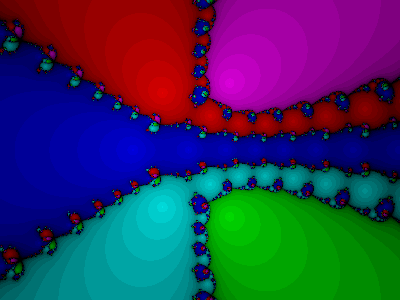
\includegraphics[scale=0.4]{figures/roots-more5} &  & 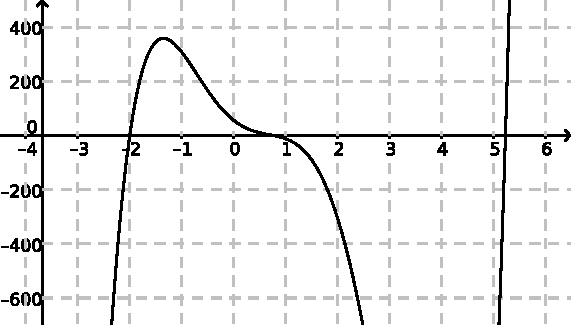
\includegraphics[scale=0.4]{figures/roots-more3}\tabularnewline
(c) &  & (d) & \tabularnewline
 & 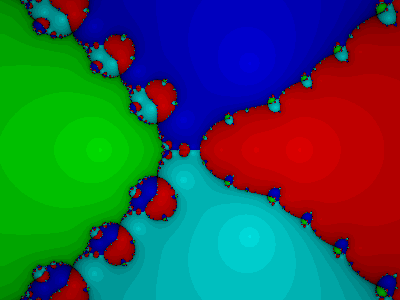
\includegraphics[scale=0.4]{figures/roots-more6} &  & 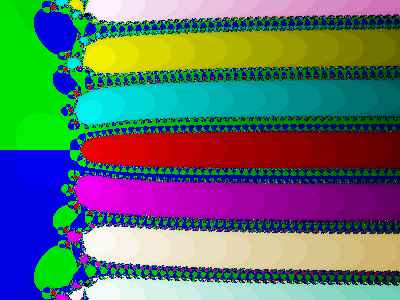
\includegraphics[scale=0.4]{figures/roots-more4}\tabularnewline
\end{tabular}
\par\end{center}
\item \label{exc:more-1}Cocokkan setiap fungsi dengan diagram kekonvergenan
metode Newton yang sesuai. Sumbu riil melintasi pusat setiap diagram,
sedangkan sumbu imajiner ditampilkan tetapi tidak selalu berada tepat
di tengah.  \hasananswer 
\begin{eqnarray*}
f(x) & = & \sin x\\
g(x) & = & \sin x-e^{-x}\\
h(x) & = & e^{x}+2^{-x}+2\cos x-6\\
l(x) & = & x^{4}+2x^{2}+4
\end{eqnarray*}

\begin{center}
\begin{tabular}{cccc}
(a) &  & (b) & \tabularnewline
 & 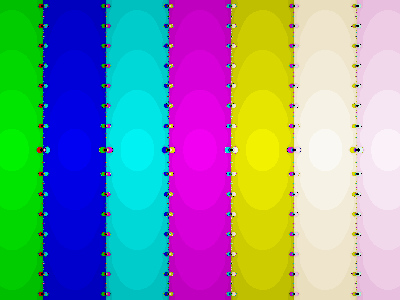
\includegraphics[scale=0.4]{figures/roots-more12} &  & 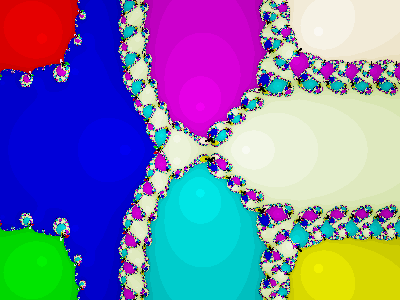
\includegraphics[scale=0.4]{figures/roots-more14}\tabularnewline
(c) &  & (d) & \tabularnewline
 & 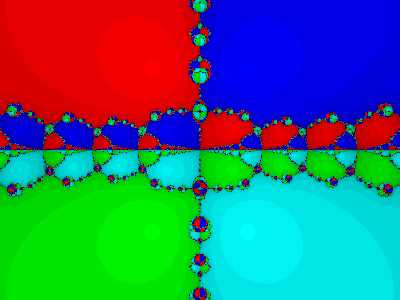
\includegraphics[scale=0.4]{figures/roots-more11} &  & 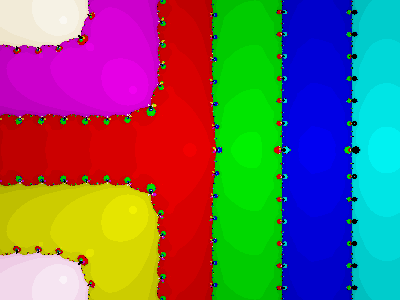
\includegraphics[scale=0.4]{figures/roots-more13}\tabularnewline
\end{tabular}
\par\end{center}
\item \label{polynomials}Tentukan sebuah polinom yang memiliki akar-akar
berikut dan tidak memiliki akar lainnya.

\begin{enumerate}
\item $-7,2,1\pm5i$
\item $-7,2,1+5i$
\item \label{exc:more-2}$-4,-1,2,\pm2i$  \hasasolution 
\item \label{exc:more-4}$-4,-1,2,2i$  \hasasolution 
\item $0,-1\pm i,1\pm i$
\item $-3+i,-2-i,-3i,1-2i$
\end{enumerate}
\item \label{newton}Buat diagram kekonvergenan metode Newton untuk polinom-polinom
pada soal \ref{polynomials}. Pastikan Anda mencakup daerah yang memperlihatkan
setidaknya area kecil yang berkonvergensi ke setiap akar. Kode Octave
dapat diunduh dari \href{http://lqbrin.github.io/tea-time-numerical/ancillaries.html}{situs pendamping}.
\item \label{noroot}Fungsi $f(x)=e^{x}$ dan $g(x)=\frac{1}{x^{2}+1}$
tidak memiliki akar, baik riil maupun kompleks. Temukan setidaknya
dua fungsi lain yang juga tidak memiliki akar.
\item \label{failure}Misalkan $f(x)=\frac{x^{2}-7x+10}{2}+\sin(3x)$.

\begin{enumerate}
\item Temukan semua akar riil dari $f$. Fungsi ini bukan polinom, sehingga
deflasi tidak dapat digunakan. Sebagai gantinya, buatlah grafik fungsi
tersebut dan gunakan metode Newton untuk menemukan akar-akarnya hingga
ketelitian $10^{-8}$. Ada empat akar. 
\item Buat diagram kekonvergenan metode Newton untuk $f$ guna melihat apakah
terdapat akar kompleks. Jika ada, gunakan metode Newton untuk menghampirinya.
Gunakan diagram kekonvergenan tersebut untuk membantu Anda memilih
nilai awal.
\item Dapatkah Anda menemukan semua akar dari $f$?
\end{enumerate}
\item \label{exc:more-3}Cocokkan setiap fungsi dengan diagram kekonvergenan
metode sekan dengan satu nilai awal yang sesuai. Sumbu riil melewati
pusat setiap diagram, sedangkan sumbu imajiner ditampilkan, tetapi
tidak selalu berada di tengah. \hasasolution  
\begin{eqnarray*}
f(x) & = & \sin x\\
g(x) & = & \sin x-e^{-x}\\
h(x) & = & e^{x}+2^{-x}+2\cos x-6\\
l(x) & = & 56-152x+140x^{2}-17x^{3}-48x^{4}+9x^{5}
\end{eqnarray*}

\begin{center}
\begin{tabular}{cccc}
(a) &  & (b) & \tabularnewline
 & 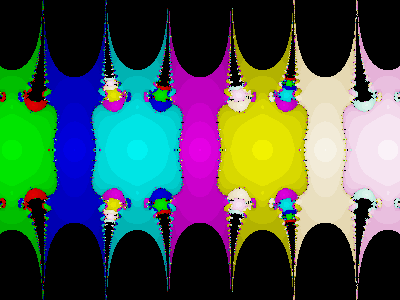
\includegraphics[scale=0.4]{figures/roots-more8} &  & 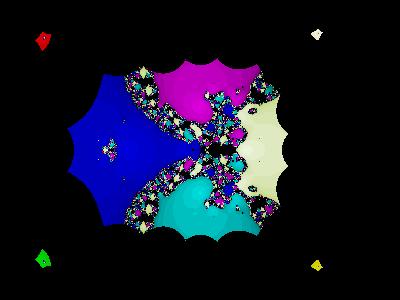
\includegraphics[scale=0.4]{figures/roots-more9}\tabularnewline
(c) &  & (d) & \tabularnewline
 & 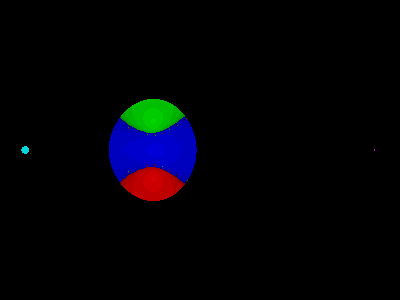
\includegraphics[scale=0.4]{figures/roots-more10} &  & 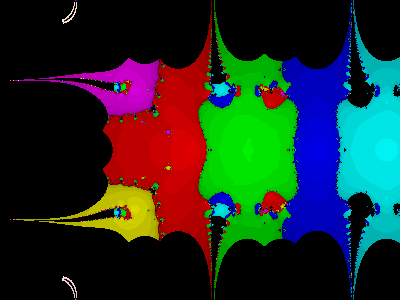
\includegraphics[scale=0.4]{figures/roots-more7}\tabularnewline
\end{tabular}
\par\end{center}
\item \label{exc:more-5}Cocokkan setiap fungsi dengan diagram kekonvergenan
metode sekan dengan satu nilai awal yang sesuai. Sumbu riil melewati
pusat setiap diagram, sedangkan sumbu imajiner ditampilkan, tetapi
tidak selalu berada di tengah. \hasananswer 
\begin{eqnarray*}
f(x) & = & x^{4}+2x^{2}+4\\
g(x) & = & (x^{2})(\ln x)+(x-3)e^{x}\\
h(x) & = & 1+2x+3x^{2}+4x^{3}+5x^{4}+6x^{5}\\
l(x) & = & (\ln x)(x^{3}+1)
\end{eqnarray*}

\begin{center}
\begin{tabular}{cccc}
(a) &  & (b) & \tabularnewline
 & 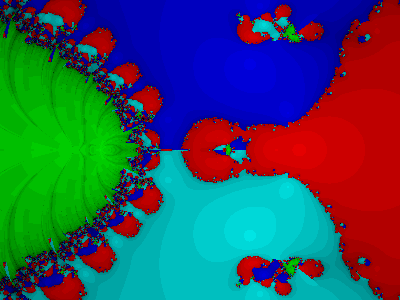
\includegraphics[scale=0.4]{figures/roots-more17} &  & 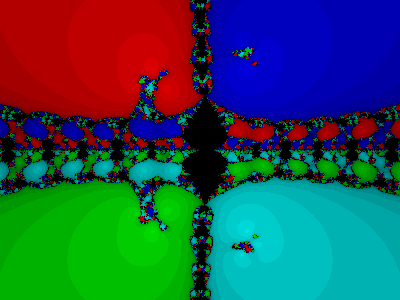
\includegraphics[scale=0.4]{figures/roots-more18}\tabularnewline
(c) &  & (d) & \tabularnewline
 & 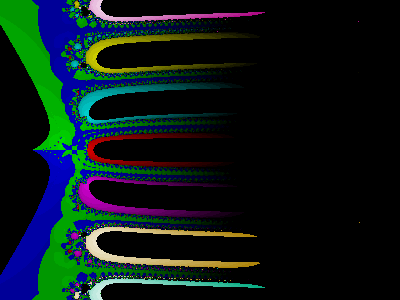
\includegraphics[scale=0.4]{figures/roots-more15} &  & 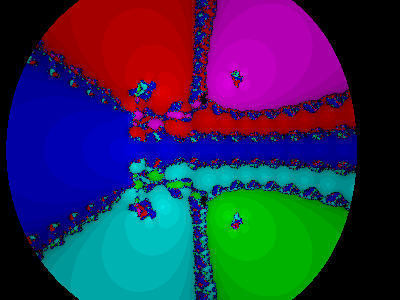
\includegraphics[scale=0.4]{figures/roots-more16}\tabularnewline
\end{tabular}
\par\end{center}
\item Buat diagram kekonvergenan metode sekan dengan satu nilai awal untuk
polinom-polinom pada soal \ref{polynomials}. Pastikan Anda mencakup
daerah yang memperlihatkan setidaknya area kecil yang berkonvergensi
ke setiap akar. Kode Octave dapat diunduh dari \href{http://lqbrin.github.io/tea-time-numerical/ancillaries.html}{situs pendamping}.
\item Diagram kekonvergenan metode Newton untuk suatu polinom sangat mirip
dengan diagram kekonvergenan metode Newton untuk polinom lainnya.
Perubahan menarik pada diagram kekonvergenan metode Newton dan diagram
kekonvergenan metode sekan dengan satu nilai awal dapat diperoleh
dengan mengalikan sebuah polinom dengan fungsi nonpolinom yang tidak
memiliki akar. Buat diagram kekonvergenan metode Newton dan diagram
kekonvergenan metode sekan dengan satu nilai awal untuk hasil kali
fungsi-fungsi pada soal \ref{polynomials} dengan fungsi-fungsi pada
soal \ref{noroot}.
\item Bahas perbandingan keunggulan dan kelemahan metode Newton, metode
sekan, dan metode sekan dengan satu nilai awal.
\end{enumerate}
\end{small}

\subsection*{Jawaban}
\begin{description}
\item [{Mengapa~ekuivalen?}] \label{que:whyEquivalent}Persamaan $g(x)=0$
dan $f(x)=x$ memiliki himpunan penyelesaian yang sama persis. $g(x)=0\Leftrightarrow1-x^{3}=0\Leftrightarrow1=x^{3}\Leftrightarrow\frac{1}{x^{2}}=x\Leftrightarrow f(x)=x$.
\item [{Bagaimana~sifat~akar-akarnya?}] \label{que:natureOfRoots} $.3181315052047641$
merupakan titik tetap dari fungsi eksponensial: \begin{verbatim}
octave:1> format('long')
octave:2> a0=.3181315052047641;
octave:3> b=sqrt(exp(2*a0)-a0^2)
b =  1.33723570143069
octave:4> exp(a0+I*b)
ans =  0.318131505204764 + 1.337235701430689i
\end{verbatim} $1.668024051576096$ merupakan titik berperiode dua dari fungsi eksponensial:
\begin{verbatim}
octave:1> format('long')
octave:2> a0=1.668024051576096;
octave:3> b=sqrt(exp(2*a0)-a0^2)
b =  5.03244706448616
octave:4> exp(a0+I*b)
ans =  1.66802405157609 - 5.03244706448616i
\end{verbatim} $2.653191974038697$ merupakan titik tetap dari fungsi eksponensial:
\begin{verbatim}
octave:5> a0=2.653191974038697;
octave:6> b=sqrt(exp(2*a0)-a0^2)
b =  13.9492083345332
octave:7> exp(a0+I*b)
ans =   2.65319197403878 + 13.94920833453319i 
\end{verbatim}
\end{description}

